\chapter{Wys-ckt的实现}\label{impl}
本章介绍本文如何根据第三章的设计完成Wys-ckt的程序实现。Wys-ckt使用Ocaml开发,类型分析程序中实现了3.2节中的类型规则,验证程序中则实现了3.3中的验证规则,完成了从Wys*程序分析、类型分析到安全计算函数编译可行性的验证的整个过程。本文实现过程中构造了两个重要的数据类型value和env帮助完成类型的分析和检查,并使用了两种语法树分别作为分析阶段和验证阶段记录程序信息的对象。
\section{结构与工具链}
本文验证系统的实现基于ML家族的Ocaml开发平台,整个实现分为三个部分如图\ref{fig:sequence}:文法分析部分,类型分析部分以及验证部分和两种语法树。
文法分析部分使用ocamllex和menhir工具进行文法分析器的编写,接受一份Wys*代码并产生该代码的语法树;类型分析部分接受前一部分产生的语法树,根据类型推导系统利用ML的模式匹配使用自建的数据结构完成对语法树的分析并产生一个带有类型的结构化信息的语法树;验证部分接受第二部分产生的更为完善的语法树,基于树中的类型信息以及验证规则通过模式匹配完成验证;完整的wys-ckt程序编译时使用ocaml-dune完成联合编译连接。
\begin{figure}[!htbp]
    \centering
    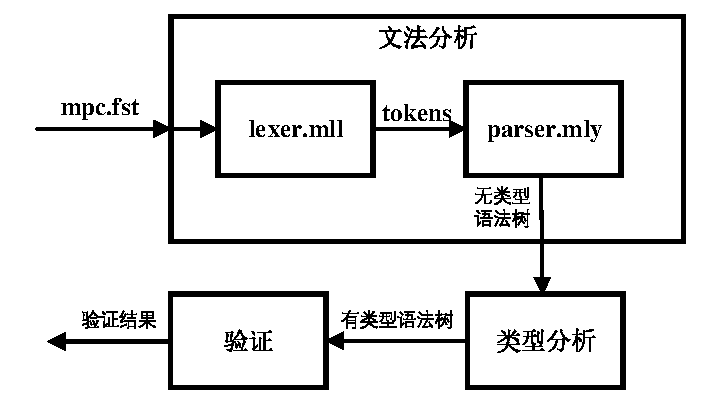
\includegraphics[width=0.70\textwidth]{sequence.pdf}
    \caption{Wys-ckt程序结构}
    \label{fig:sequence}
\end{figure}

Wys-ckt作为一环插入在整个程序验证部署环节当中,它接受一个经过Fstar验证的Wys*程序,验证完成后再经Fstar将程序编译为Ocaml或Fsharp目标代码,然后经由对应平台编译运行,Wys-ckt在整个验证部署环节中所处的位置如图\ref{fig:position_sequence}。

\begin{figure}[!htbp]
    \centering
    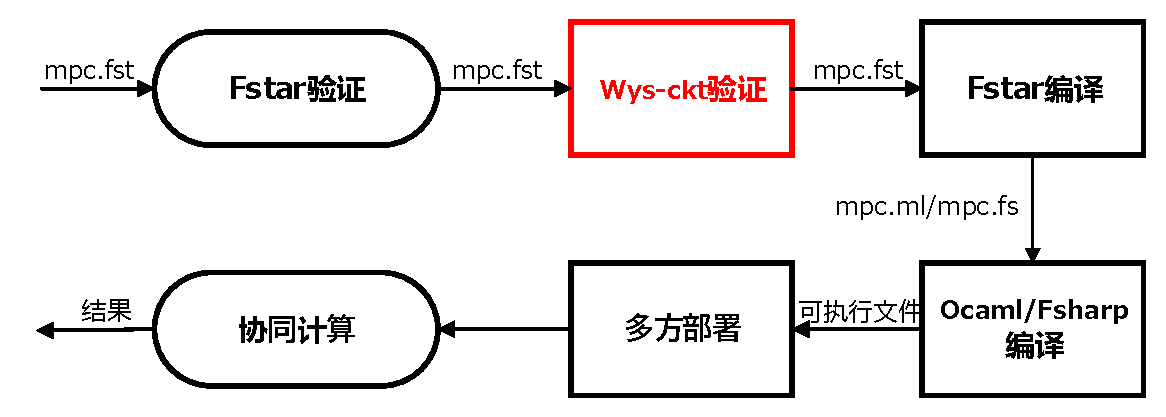
\includegraphics[width=1.00\textwidth]{sequence_all.pdf}
    \caption{Wys-ckt在Wys*程序验证部署流程中所处的位置}
    \label{fig:position_sequence}
\end{figure}

整个Wys-ckt的程序实现包含了大约500行Ocaml有效代码的文法分析部分,800行有效代码的语法树与类型分析部分,300行有效代码的验证部分,Wys-ckt的实际程序实现可以访问我的个人仓库https://github.com/YuXinFan/Wys-ckt获取。
\section{主要数据结构}
本文主要的数据结构包括两种语法树以及用于类型推导的记录结构化数据value和类型分析环境env。在一个纯函数式的程序当中的所有数值、变量、函数等元素都被看作与特定值绑定的命名量,因此声明一个如图\ref{fig:dvalue}结构式记录数据value记录每个命名量所绑定的值类型与所属的上下文环境。value中包含丰富的信息,每一个通过声明产生的变量都有一个value记录下它的名,所属类型,所属的环境,所包含的语法树。当通过声明产生一个函数时,value会额外记录函数的参数类型,返回类型,以及函数定义。value被用作有类型语法树重要基础组成,使有类型语法树包含了更丰富的信息。 
\begin{figure}[!htbp]
    \centering
    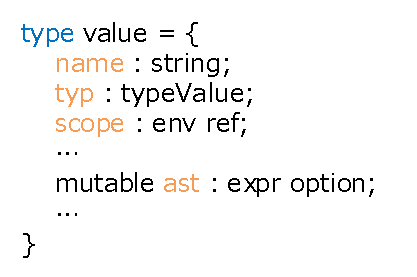
\includegraphics[width=0.50\textwidth]{dvalue.pdf}
    \caption{value结构记录的部分内容}
    \label{fig:dvalue}
\end{figure}
另一个结构式数据env如图\ref{fig:env}被用作类型分析时的环境,env中记录当前域的标识符和包含的所有类型作用域,一个env数据中不仅包含了当前环境的value数据、子作用域的env数据还记录了不同作用域之间的相对关系。当类型分析需要查询已有的命名变量的类型时,可以以名为关键字在当前环境和外部环境的env中查询获得所需要的信息。Wys-ckt通过创建一个拥有Env类型的只包含一个类型环境env字段的value数据,达到区别不同环境和变量在整个程序中所属的相对位置的目的。
\begin{figure}[!htbp]
    \centering
    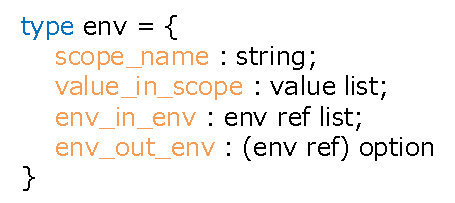
\includegraphics[width=0.50\textwidth]{env.pdf}
    \caption{env记录结构包含的字段}
    \label{fig:env}
\end{figure}
\section{语法树}
本部分分为三个阶段,第一阶段基于文法分析产生一个包含尽量多信息的预分析无类型语法树;第二阶段基于无类型语法树与类型推导规则进行类型推导;第三阶段重构一个结构更为清晰的有类型语法树。
\subsection{无类型语法树}
无类型语法树的构成有四层,程序层、声明层、表达式与类型声明层、命名变量层,每一层都按照文法规则设计,与3.1节中的语法一一对应。一个\textbf{module}语法与一系列decl声明语法共同组成一个完整的程序层。声明层包含四种声明分别对应\textbf{open}、\textbf{val}、\textbf{type}和\textbf{let}声明。表达式与类型声明层包含所有表达式种类以及函数定义时的参变量类型标识。命名变量层则用于记录变量、常数、匿名函数。

无类型语法树在文法分析过程中进行构建。分析一个Wys*的文法时会自动构建出一个分析树,这个分析树的结构与语法树对应。让文法分析树在每一个节点结束时生成一个对应结构的语法树节点,文法分析完成的同时一个无类型语法树也构建完成。
\subsection{静态类型分析}
无类型语法树中包含了一部分粗粒度处理过的信息(层级,表达式种类等)以及大部分的原始信息,这些信息需要加工后才能用于后续的分析工作,因此该部分的作用在于将其中的信息(尤其是类型信息)进行细化处理分类并进行按照类型推导规则填补空缺。

4.2节中数据结构主要就是为了解决这一部分问题,此部分的实现方法基于3.2节中的类型推导规则完成。所有的类型构建为一个联合结构,使用不同的类型名加以区分,然后遍历无类型语法树的每一个节点,按照3.2节的类型推导规则进行分析推导。对于一个叶节点上的值,首先匹配其模式是否为常数类型模式,如果是常数类型则按照所对应的模式分配类型,否则认为是一个命名变量类型。一个新的命名变量$v$由\textbf{let}声明或\textbf{let} \textbf{in}表达式产生,分析出它的类型等信息后将其名、类型、作用域、结构等信息组合成一个4.2中的value数据,并存入当前类型分析环境env中。当类型分析需要时,以名为关键字在当前环境中向上搜索即可得到包含$v$的所有信息在内的value数据。

在类型分析的过程中,对表达式层的分析占大部分内容。算法\ref{alg:exprtype}介绍本文实现的表达式层进行类型分析的方法。在算法\ref{alg:exprtype}中,\Call{TypeExpr}{}接受一个无类型语法树$ast$和类型环境$env$,返回$ast$的类型结果。\Call{TypeExpr}{}先从$ast$中获取根节点代表的表达式类型和各个子表达式,然后调用3.2节中描述的类型规则的具体实现函数\Call{TypeRule}{}完成类型推导。如3.2节中所描述的,\Call{TypeRule}{}包含每一种表达式的类型推导方法,由于篇幅原因本文算法\ref{alg:typerule}只展示\Call{TypeRule}{}的一部分内容。
\begin{algorithm}[!htbp]
    \small
    \caption{Expression Type Analysis Algorithm}\label{alg:exprtype}
    \hspace*{0.02in} {\bf Input:} \\
	\hspace*{0.04in} $ast$: The type-free abstract tree of the content of program \\
	\hspace*{0.04in} $env$: The typing environment containing types, methods, scopes \\
	\hspace*{0.02in} {\bf Output:} \\
	\hspace*{0.04in} The result type of the input expression
    \begin{algorithmic}[1]
        \Procedure{TypeExpr}{$env,ast$}
        \State $p\gets \text{pattern of } ast$ \Comment{获取输入表达式语法树$ast$的类型$p$}
        \State $m\gets \text{children of } ast$ \Comment{获得输入表达式语法树$ast$的所有次一级子树$m$}
        \State \Return \Call{TypeRule}{$env$,$p$,$m$} \Comment{调用类型推导规则的实现函数获得类型}
        \EndProcedure
    \end{algorithmic}
\end{algorithm}
\begin{algorithm}[!htbp]
    \small
    \caption{Partial of Type Rule Algorithm}\label{alg:typerule}
     \hspace*{0.02in} {\bf Input:} \\
	\hspace*{0.04in} $env$: The typing environment containing types, methods, scopes \\
	\hspace*{0.04in} $p$: The pattern expression type of an expression \\
	\hspace*{0.04in} $m$: A tuple containing abstract tree of sub-expressions \\
	\hspace*{0.02in} {\bf Output:} \\
	\hspace*{0.04in} The result type inferred from inputs
    \begin{algorithmic}[1]
        \Procedure{TypeRule}{$env,p,m$}
        \If {$p$=Constant}
        \State $c\gets \text{first of } m$ \Comment{从元组$m$中取得元素,常数节点$c$}
        \State \Return \Call{TypeConstant}{$c$} \Comment{匹配常数类型}
        \ElsIf {$p$=Variable}
        \State $x\gets \text{first of } m$ \Comment{从元组$m$中取得元素,变量节点$x$}
        \State \Return \Call{Find}{$env$,$x$}$.type$ \Comment{从env中查找$x$,并获得$x$的类型}
        \ElsIf {$p=$LetIn}
        \State $(x,e_1,e_2)\gets m$
        \State $env_2\gets env.sub\_env()$ \Comment{创建一个子环境}
        \State $env_2.value[x]\gets$ \Call{TypeExpr}{$env$, $e_1$}\Comment{在子环境中增加$x$对应的类型}
        \State \Return \Call{TypeExpr}{$env_2$, $e_2$} \Comment{LetIn表达式的类型取决于$e_2$}
        \ElsIf {$p=$IfCondition}
        \State $(b,e_1,e_2)\gets m$
        \State $typ \gets $\Call{TypeExpr}{$b$}
        \State $env_1\gets env.sub\_env()$ \Comment{创建子环境}
        \State $typ_1\gets$ \Call{TypeExpr}{$env_1$,$e_1$}\Comment{在子环境进行$e_1$的类型分析}
        \State $env_2\gets env.sub\_env()$
        \State $typ_2\gets$ \Call{TypeExpr}{$env_2$,$e_2$}
        \State \Return $typ_1$
        \ElsIf {...}
        \State {...}
        \EndIf 
        \EndProcedure
    \end{algorithmic}
\end{algorithm}
\subsection{有类型语法树}
有类型的语法树与无类型语法树的不同在于基础节点由原始字符信息变更为信息更为完整的value数据并且枝剪了不必要的细化类型信息。有类型语法树的结构框架仍依照无类型语法树,静态分析时产生的各个value数据不断填补到语法树的对应位置即能完成有类型语法树的构建。
\section{验证函数}
获得完整的有类型信息的语法树之后,得益于ML家族的模式匹配特性,验证函数的实现过程十分方便。\Call{CheckingRule}{}实现了3.3节中描述的不同表达式所受到的类型限制的检查,\Call{CheckingRule}{}也使用模式匹配和分支的结构,与算法\ref{alg:typerule}的形式类似。算法\ref{alg:verify}描述了对安全计算函数进行验证的方法。在完整的验证过程中,Wys-ckt通过遍历搜索定位程序中的\textbf{as\_sec} $ps$ $g$语句,$g$即为待验证的安全计算函数的名,然后以$g$为关键字在语句所在的上下文环境中找出$g$所定义的表达式内容,该表达式对应的语法树$ast$即为待验证的安全计算函数表达式的等价语法树,$ast$将作为函数输入参数传递给验证函数verify\_as\_sec。verify\_as\_sec调用算法\ref{alg:verify}和\Call{CheckingRule}{}的实际实现函数verify\_ast\_expr完成对安全计算函数的验证。
\begin{algorithm}[!htbp]
    \small
    \caption{Verification Algorithm}\label{alg:verify}
    \hspace*{0.02in} {\bf Input:} \\
	\hspace*{0.04in} $ast$: the typed abstract tree of the content of secure function \\
	\hspace*{0.02in} {\bf Output:} \\
	\hspace*{0.04in} $true$ means succeed,vice versa.
    \begin{algorithmic}[1]
        \Procedure{VerifyExpr}{$ast$}
        \State $p\gets \text{pattern of } ast$ \Comment{获取表达式语法树$ast$的类型$p$}
        \State $m\gets \text{children of } ast$ \Comment{获取表达式语法树$ast$的所有次一级子树$m$}
        \State $r\gets$ \Call{CheckingRule}{$p$,$m$} \Comment{调用验证规则算法检查$m$和$p$是否符合验证规则}
        \For{each subtree $i$ in $m$}
        \State $s\gets$ \Call{VerifyExpr}{$i$} \Comment{依次验证每一个子表达式}
        \If {$s=false$}
        \State \Return $false$
        \EndIf
        \EndFor
        \State \Return $r$
        \EndProcedure
    \end{algorithmic}
\end{algorithm}